\begin{SCn}

\scnsectionheader{\currentname}

\scnstartsubstruct
	
\scnheader{интерфейсное действие пользователя}
\scnaddlevel{1}
\scnidtf{user interface action}
\scnaddlevel{-1}
	\scnsuperset{действие мышью}
	\scnaddlevel{1}
	\scnidtf{mouse-action}
	\scnaddlevel{-1}
		\scnaddlevel{1}
		\scnsuperset{прокрутка мышью}
		\scnaddlevel{1}
		\scnidtf{mouse-scroll}
		\scnaddlevel{-1}
			\scnaddlevel{1}
			\scnsuperset{прокрутка мышью вверх}
			\scnaddlevel{1}
			\scnidtf{mouse-scroll-up}
			\scnaddlevel{-1}
			\scnsuperset{прокрутка мышью вниз}
			\scnaddlevel{1}
			\scnidtf{mouse-scroll-down}
			\scnaddlevel{-1}
			\scnaddlevel{-1}
		\scnsuperset{наведение мышью}
		\scnaddlevel{1}
		\scnidtf{mouse-hover}
		\scnaddlevel{-1}
		\scnsuperset{отпускание мышью}
		\scnaddlevel{1}
		\scnidtf{mouse-drop}
		\scnaddlevel{-1}
		\scnsuperset{нажатие мыши}
		\scnaddlevel{1}
		\scnidtf{mouse-click}
		\scnaddlevel{-1}
			\scnaddlevel{1}
			\scnsuperset{одиночное нажатие мыши}
			\scnaddlevel{1}
			\scnidtf{mouse-single-click}
			\scnaddlevel{-1}
			\scnsuperset{двойное нажатие мыши}
			\scnaddlevel{1}
			\scnidtf{mouse-double-click}
			\scnaddlevel{-1}			
			\scnaddlevel{-1}
		\scnsuperset{жест мышью}
		\scnaddlevel{1}
		\scnidtf{mouse-gesture}
		\scnaddlevel{-1}
		\scnsuperset{отведение мышью}	
		\scnaddlevel{1}
		\scnidtf{mouse-unhover}
		\scnaddlevel{-1}	
		\scnsuperset{перетаскивание мышью}
		\scnaddlevel{1}
		\scnidtf{mouse-drag}
		\scnaddlevel{-1}
		\scnaddlevel{-1}		
	\scnsuperset{действие голосом}
	\scnaddlevel{1}
	\scnidtf{speech-action}
	\scnaddlevel{-1}
	\scnsuperset{действие клавиатурой}
	\scnaddlevel{1}
	\scnidtf{keyboard-action}
	\scnaddlevel{-1}
			\scnaddlevel{1}
			\scnsuperset{нажатие функциональной клавиши}
			\scnaddlevel{1}
			\scnidtf{press-function-key}
			\scnaddlevel{-1}
			\scnsuperset{нажатие клавиши набора текста}
			\scnaddlevel{1}
			\scnidtf{type-text}
			\scnaddlevel{-1}
			\scnaddlevel{-1}	
	\scnsuperset{действие осязанием}
	\scnaddlevel{1}
	\scnidtf{tangible-action}
	\scnaddlevel{-1}	
	\scnsuperset{действие сенсором}	
	\scnaddlevel{1}
	\scnidtf{touch-action}
	\scnaddlevel{-1}
		\scnaddlevel{1}
		\scnsuperset{нажатие сенсора}
		\scnaddlevel{1}
		\scnidtf{touch-click}
		\scnaddlevel{-1}
			\scnaddlevel{1}
			\scnsuperset{одиночное нажатие сенсора}
			\scnaddlevel{1}
			\scnidtf{touch-single-click}
			\scnaddlevel{-1}
			\scnsuperset{двойное нажатие сенсора}
			\scnaddlevel{1}
			\scnidtf{touch-double-click}
			\scnaddlevel{-1}
			\scnaddlevel{-1}
		\scnsuperset{жест по сенсору}
		\scnaddlevel{1}
		\scnidtf{touch-gesture}
		\scnaddlevel{-1}
			\scnaddlevel{1}
			\scnsuperset{жест по сенсору одним пальцем}
			\scnaddlevel{1}
			\scnidtf{one-fingure-gesture}
			\scnaddlevel{-1}
			\scnsuperset{жест по сенсору несколькими пальцами}
			\scnaddlevel{1}
			\scnidtf{multiple-finger-gesture}
			\scnaddlevel{-1}
			\scnaddlevel{-1}
		\scnsuperset{отпускание сенсором}
		\scnaddlevel{1}
		\scnidtf{touch-drop}
		\scnaddlevel{-1}
		\scnsuperset{перетаскивание сенсором}
		\scnaddlevel{1}
		\scnidtf{touch-drag}
		\scnaddlevel{-1}
		\scnaddlevel{-1}
	\scnsuperset{действие пером}
	\scnaddlevel{1}
	\scnidtf{pen-base-action}
	\scnaddlevel{-1}	
		\scnaddlevel{1}
		\scnsuperset{нажатие функциональной клавиши пером}
		\scnaddlevel{1}
		\scnidtf{touch-function-key}
		\scnaddlevel{-1}
		\scnsuperset{рисование пером}
		\scnaddlevel{1}
		\scnidtf{draw}
		\scnaddlevel{-1}
		\scnsuperset{написание текста пером}
		\scnaddlevel{1}
		\scnidtf{write-text}
		\scnaddlevel{-1}
		\scnaddlevel{-1}
		
		
\scnheader{прокрутка мышью}
\scnexplanation{\textit{прокрутка мышью} -- интерфейсное действие пользователя, соответствующее прокрутке содержимого некоторого компонента пользовательского интерфейса при помощи мыши.}

\scnheader{наведение мышью}
\scnexplanation{\textit{наведение мышью} -- интерфейсное действие пользователя, соответствующее появлению курсора мыши в рамках компонента пользовательского интерфейса.}

\scnheader{отпускание мышью}
\scnexplanation{\textit{отпускание мышью} -- интерфейсное действие пользователя, соответствующее отпусканию некоторого компонента пользовательского интерфейса в рамках другого компонента пользовательского интерфейса при помощи мыши.}

\scnheader{нажатие мыши}
\scnexplanation{\textit{нажатие мыши} -- интерфейсное действие пользователя, соответствующее выполнению нажатия мыши в рамках некоторого компонента пользовательского интерфейса.}

\scnheader{отведение мышью}
\scnexplanation{\textit{отведение мышью} -- интерфейсное действие пользователя, соответствующее выходу курсора мыши за рамки компонента пользовательского интерфейса.}

\scnheader{перетаскивание мышью}
\scnexplanation{\textit{перетаскивание мышью} -- интерфейсное действие пользователя, соответствующее перетаскиванию компонента пользовательского интерфейса при помощи мыши.}

\scnheader{нажатие сенсора}
\scnexplanation{\textit{нажатие сенсора} -- интерфейсное действие пользователя, соответствующее выполнению нажатия сенсора в рамках некоторого компонента пользовательского интерфейса.}

\scnheader{жест по сенсору}
\scnexplanation{\textit{жест по сенсору} -- интерфейсное действие пользователя, соответствующее выполнению некоторого жеста, выполняемого при помощи движения пальцев на экране сенсора.}

\scnheader{отпускание сенсором}
\scnexplanation{\textit{отпускание сенсором} -- интерфейсное действие пользователя, соответствующее отпусканию некоторого компонента пользовательского интерфейса в рамках другого компонента пользовательского интерфейса при помощи сенсора.}

\scnheader{перетаскивание сенсором}
\scnexplanation{\textit{перетаскивание сенсором} -- интерфейсное действие пользователя, соответствующее перетаскиванию компонента пользовательского интерфейса при помощи сенсора.}

\scnheader{действие пером}
\scnexplanation{\textit{действие пером} -- интерфейсное действие пользователя, осуществляемое при помощи пера на графическом планшете.}

\scnheader{инициируемое пользовательским интерфейсом действие*}
\scniselement{квазибинарное отношение}
\scniselement{ориентированное отношение}
\scnrelfrom{первый домен}{компонент пользовательского интерфейса $\cup$ user interface action class}
\scnrelfrom{второй домен}{класс внутренних действий системы}
\scnrelfrom{иллюстрация}{
	\scnfileimage{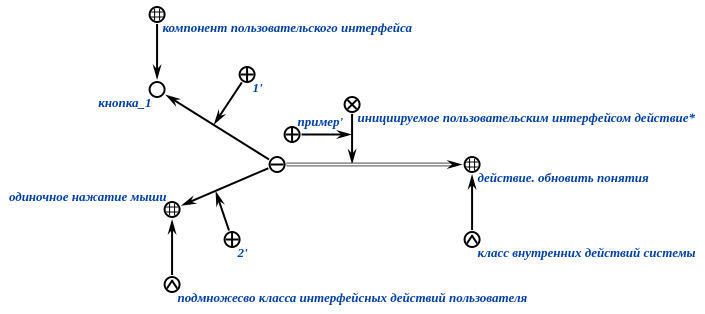
\includegraphics[width=1\linewidth]{figures/sd_ui/ui_initiated_action.png}}}

\scnendstruct \scnendcurrentsectioncomment

\end{SCn}